\chapter{Практические задания}
\section{Задание №1}
\textbf{Задание:} составить базу знаний <<Собственники>>, дополнив (и минимально изменив) базу знаний, хранящую знания.
\begin{itemize}
	\item \textbf{<<Телефонный справочник>>}: Фамилия, №тел, Адрес -- структура (Город, Улица, №дома, №кв);
	\item \textbf{<<Автомобили>>}: Фамилия\_владельца, Марка, Цвет, Стоимость и др.;
	\item \textbf{<<Вкладчики банков>>}: Фамилия, Банк, счет, сумма, др.
\end{itemize}
знаниями о дополнительной собственности владельца. Преобразовать знания об автомобиле к форме знаний о собственности.

Вид собственности (кроме автомобиля):
\begin{itemize}
	\item строение, стоимость и другие его характеристики;
	\item участок, стоимость и другие его характеристики;
	\item водный\_транспорт, стоимость и другие его характеристики.
\end{itemize}

Описать и использовать вариантный домен: Собственность. Владелец может иметь, но только один объект каждого вида собственности (это касается и автомобиля), или не  иметь некоторых видов собственности. Обеспечить возможность поиска.
\begin{enumerate}
	\item Названий всех объектов собственности заданного субъекта.
	\item Названий и стоимости всех объектов собственности заданного субъекта.
	\item * Разработать правило, позволяющее найти суммарную стоимость всех объектов собственности заданного субъекта.
\end{enumerate}

Для 2-ого пункта и одной фамилии составить таблицу, отражающую конкретный порядок работы системы с объяснениями порядка работы и особенностей использования доменов (указать конкретные T1 и T2 и полную подстановку на каждом шаге). При желании можно усложнить базу знаний, введя варианты: строение: (Дом, офис, торговый центр), участок: (садовый, территория на застройку, территория под агро-работы), водный\_транспорт: варианты названий.

Код программы представлен на листинге \ref{lst:code}.

\begin{lstlisting}[label=lst:code, basicstyle=\footnotesize, caption=Код программы]
domains
	%general for all
	price = integer
	
	%phone
	surname = string
	phone_number = string
	city = string
	street = string
	house_number = integer
	flat_number = integer
	struct_address = address(city, street, house_number, flat_number)
	
	%cars
	car_brand = string
	car_color = string
	
	%bank depositor
	bank_name = string
	bank_account = string
	account_cost = integer
	
	%property owner
	property_name = string
	type = symbol
	property = building(property_name, type, price);
	plot(property_name, type, price);
	water_transport(property_name, type, price);
	car(property_name, car_brand, car_color, price)
	
predicates
	phone(surname, phone_number, struct_address).
	bank_depositor(surname, bank_name, bank_account, account_cost).
	owner(surname, property).
	
	find_info_name_properties(surname, surname, property_name).
	find_info_name_price_properties(surname, surname, property_name, price).
	find_sum(surname, result_price).
	find_sum_price_properties(surname, result_price).
	if_property(surname, type, price).
clauses
	phone("Pavlov", "+7(934)245-34-12", 
			address("Moscow", "St.1905 year", 20, 154)).
	phone("Pavlov", "+7(924)056-78-34",
			address("Moscow", "St.1905 year", 20, 154)).
	phone("Dremin", "+7(984)874-91-23",
			address("Moscow", "Tverskaya", 53, 26)).
	phone("Agafonova", "+7(934)812-38-47", 
			address("Moscow", "Bolshaya Dmitrovka", 7, 15)).
	phone("Agafonova", "+7(956)361-31-17", 
			address("Moscow", "Bolshaya Dmitrovka", 7, 15)).
	
	owner("Pavlov", car("TC", "Toyota Camry", "Silver", 1200000)).
	owner("Pavlov", car("HO", "Honda Oddysey", "Black", 900000)).
	owner("Dremin", car("FM", "Ford Mustang", "Blue", 1800000)).
	owner("Pavlov", building("Home", flat, 15200)).
	owner("Dremin", water_transport("Jetmax", speedboat, 180000)).
	owner("Agafonova", plot("Greenland", speedboat, 9635000)).
	
	bank_depositor("Agafonova", "Sberbank", "0401-2535", 15000).
	bank_depositor("Agafonova", "Tinkoff", "1431-5836", 25000).
	bank_depositor("Dremin", "VTB", "9631-7521", 20000).
	bank_depositor("Pavlov", "Alpha", "9631-7521", 20000).
	
	if_property(Surname, car, Price) :- owner(Surname, car(_, _, _, Price)), !.
	if_property(Surname, building, Price) :- 
		owner(Surname, building(_, _, Price)), !.
	if_property(Surname, water_transport, Price) :- 
		owner(Surname, water_transport(_, _, Price)), !.
	if_property(Surname, plot, Price) :- owner(Surname, plot(_, _, Price)), !.
	if_property(_, _, 0).
	
	find_sum(Surname, Sum_price) :- 
		if_property(Surname, car, Car_price),
		if_property(Surname, building, Building_price),
		if_property(Surname, water_transport, Water_transport_price),
		if_property(Surname, plot, Plot_price),
		Sum_price = Car_price + Building_price + Water_transport_price + Plot_price.  							  
	
	find_info_name_properties(Surname, Surname, Property_name) :- 
		owner(Surname, car(Property_name, _, _, _)).
	find_info_name_properties(Surname, Surname, Property_name) :- 
		owner(Surname, building(Property_name, _, _)).
	find_info_name_properties(Surname, Surname, Property_name) :-
		owner(Surname, water_transport(Property_name, _, _)).
	find_info_name_properties(Surname, Surname, Property_name) :-
		owner(Surname, plot(Property_name, _, _)).
	
	find_info_name_price_properties(Surname, Surname, Property_name, Price) :- owner(Surname, car(Property_name, _, _, Price)).
	find_info_name_price_properties(Surname, Surname, Property_name, Price) :- owner(Surname, building(Property_name, _, Price)).
	find_info_name_price_properties(Surname, Surname, Property_name, Price) :- owner(Surname, water_transport(Property_name, _, Price)).
	find_info_name_price_properties(Surname, Surname, Property_name, Price) :- owner(Surname, plot(Property_name, _, Price)).
	
	find_sum_price_properties(Surname, Sum_price) :-
		find_sum(Surname, Sum_price).								       
goal
	%Вопрос для пункта 1
	%find_info_name_properties("Dremin", Surname, Property_name).
	
	%Вопрос для пункта 2
	%find_info_name_price_properties("Dremin", Surname, Property_name, Price). 
	
	%Вопрос для пункта 3
	%find_sum_price_properties("Dremin", Sum_price). 
\end{lstlisting}

Ниже на рисунках \ref{image:table_1} и \ref{image:table_2} приведена таблица порядка поиска ответов для второго пункта задания:
\begin{figure}[H]
	\centering{
		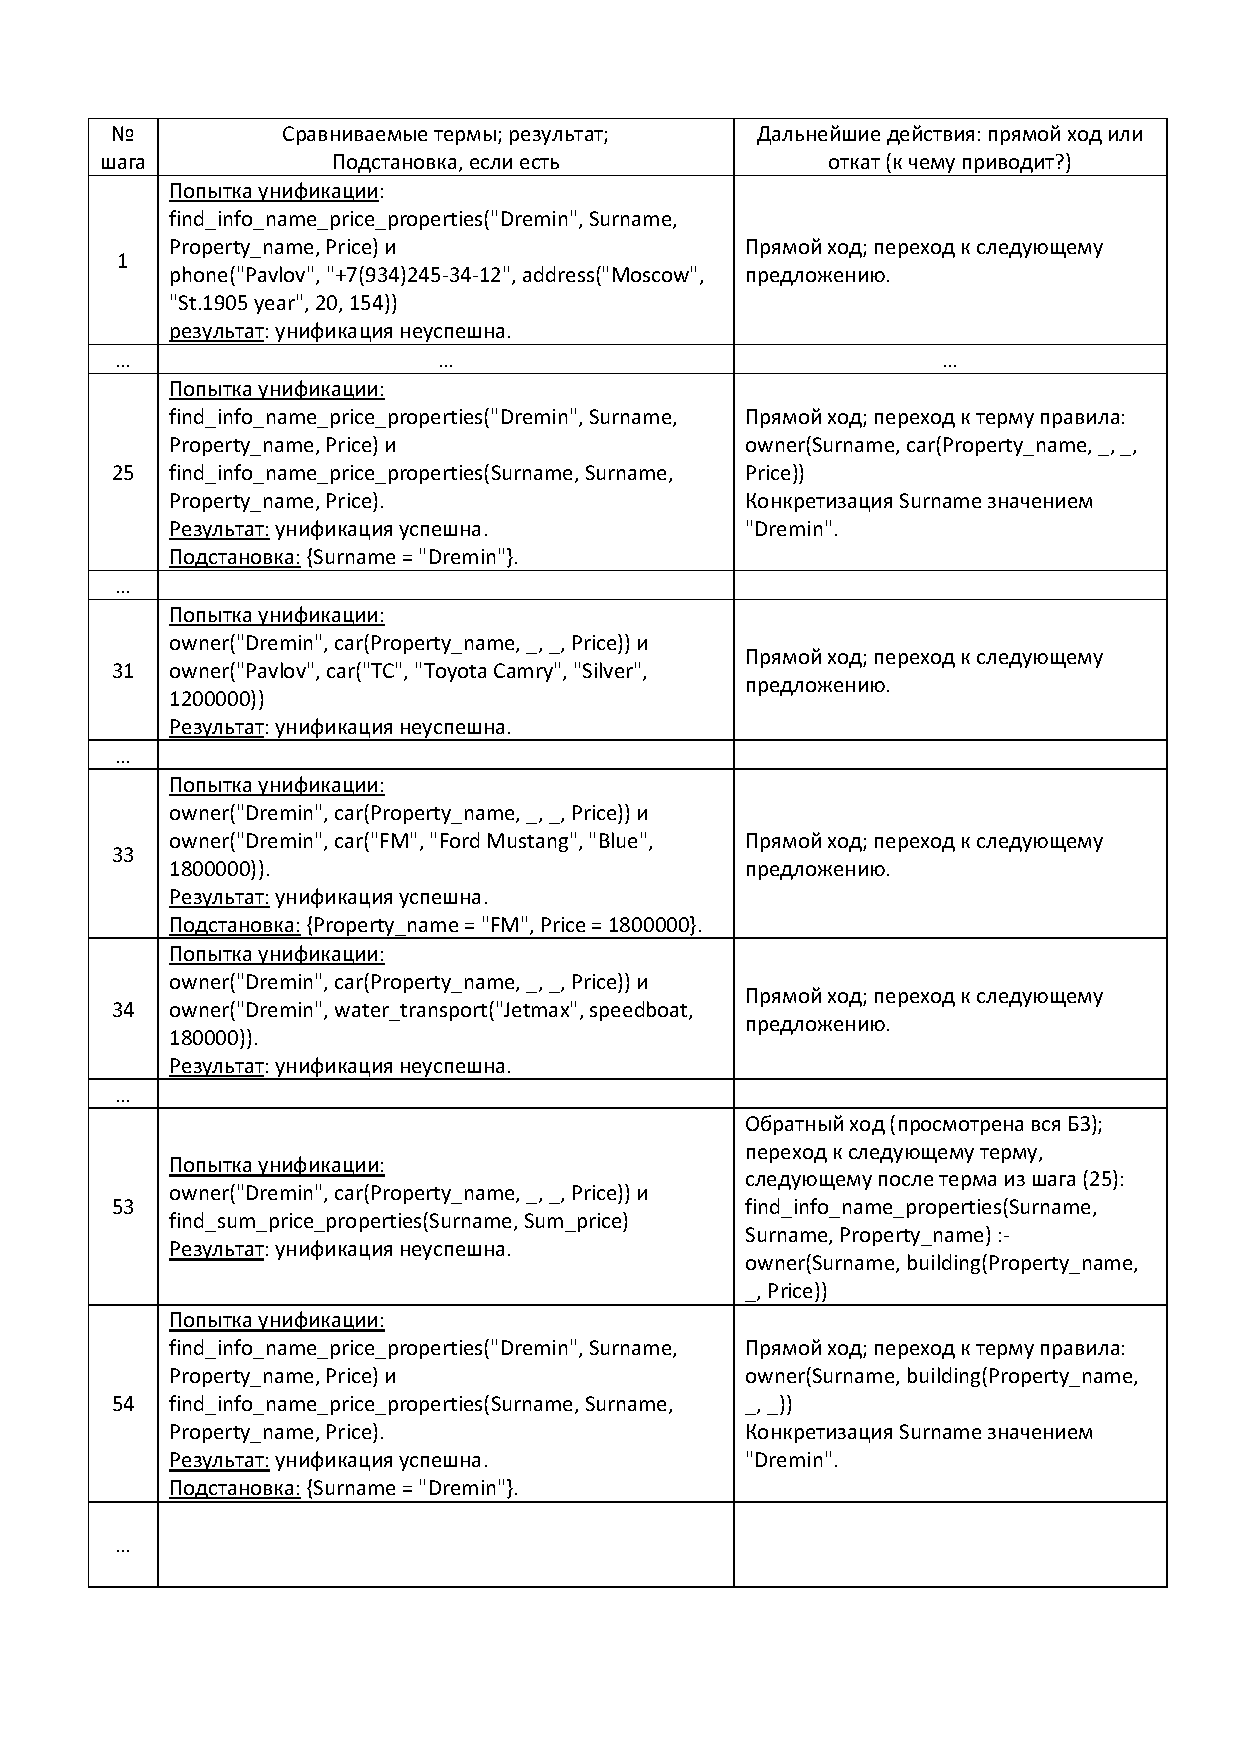
\includegraphics[scale=0.93]{images/table_3_1.pdf}
		\caption{Таблица порядка поиска ответов для второго пункта задания.}
		\label{image:table_1}
	}
\end{figure}

\begin{figure}[H]
	\centering{
		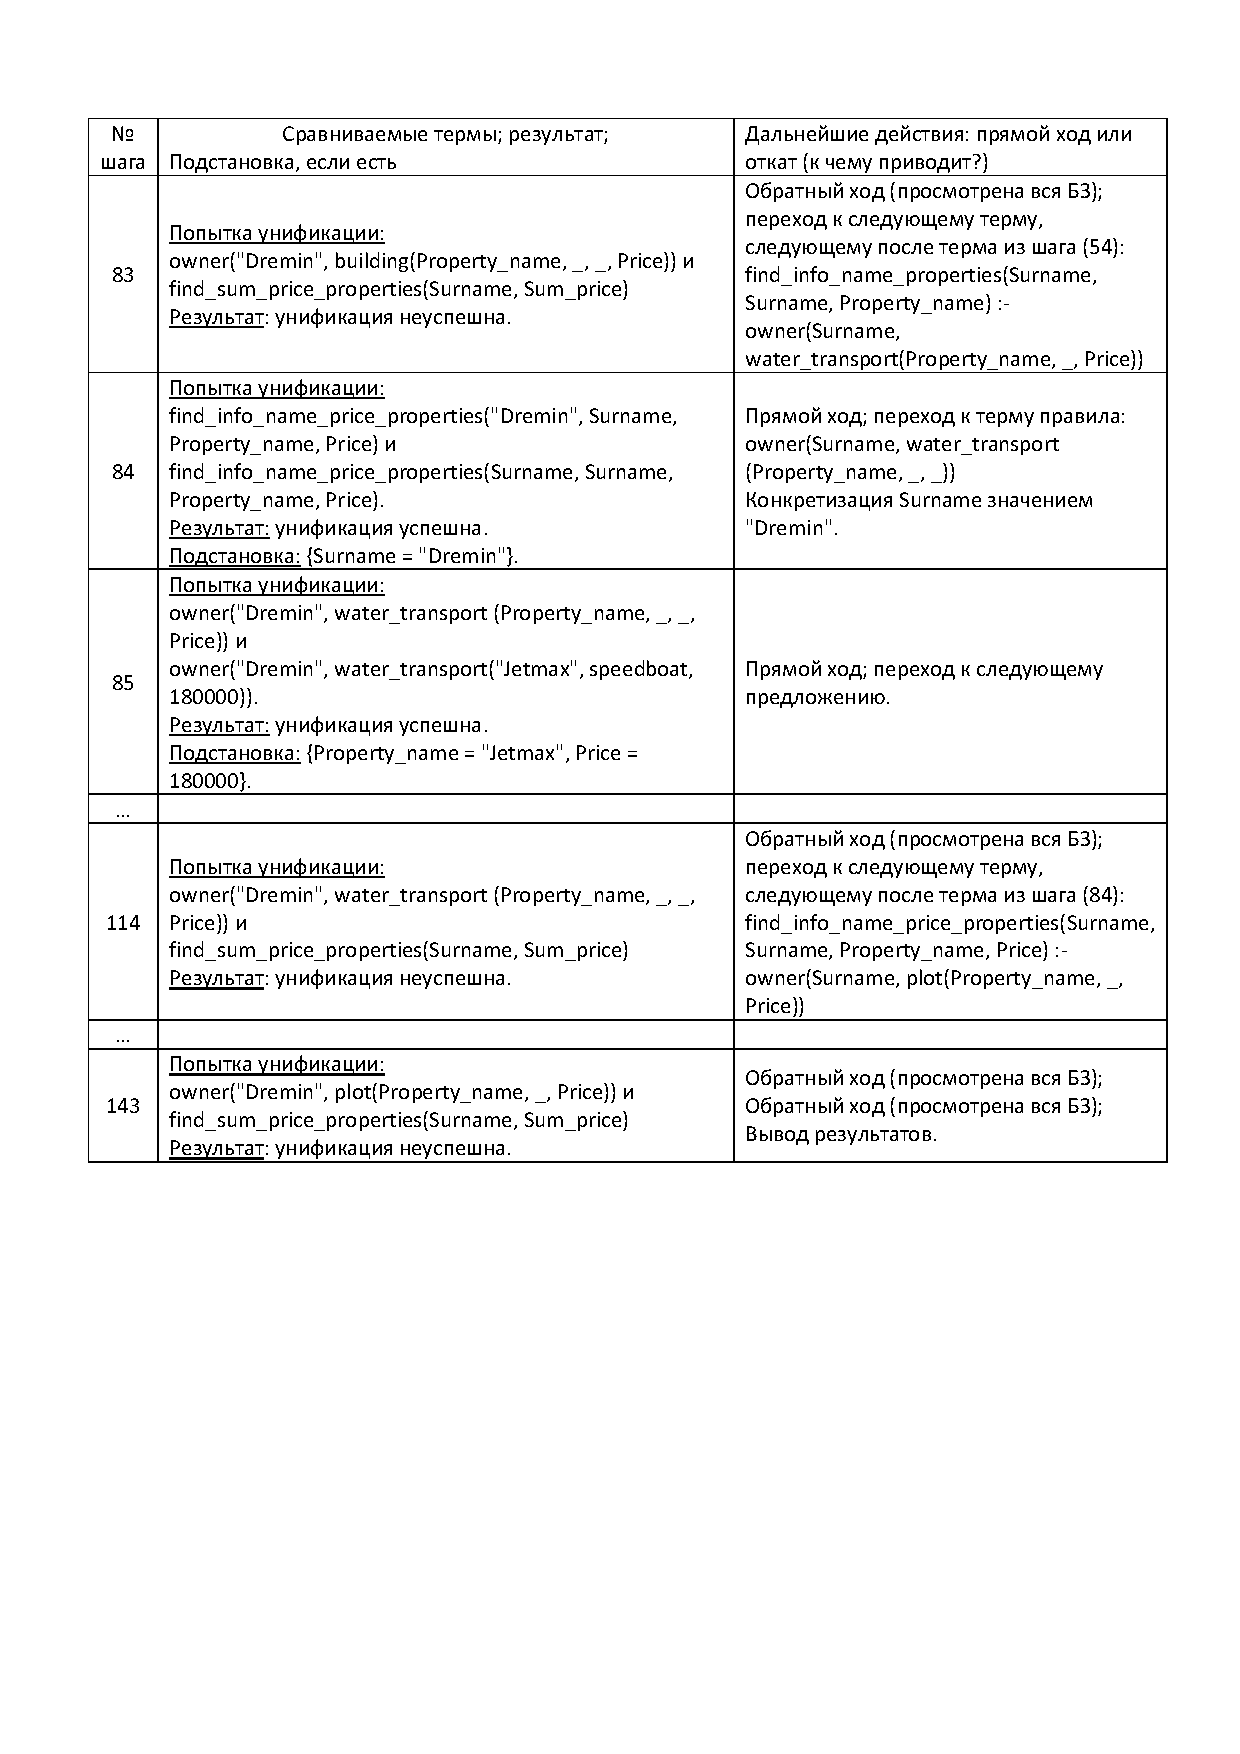
\includegraphics[scale=0.93]{images/table_3_2.pdf}
		\caption{Таблица порядка поиска ответов для второго пункта задания (продолжение)}
		\label{image:table_2}
	}
\end{figure}
